\documentclass[a4paper]{article}
\usepackage{sbc-template}
\usepackage[brazilian]{babel}
\usepackage[utf8]{inputenc}
\usepackage[T1]{fontenc}
\usepackage{enumerate}
\usepackage{color}
\usepackage{listings}
\usepackage{graphicx}
\usepackage{float}
\usepackage{hyperref}
\usepackage{amsmath}
\usepackage{morefloats}

\graphicspath{{figures/}}
\definecolor{dkgreen}{rgb}{0,0.6,0}
\definecolor{gray}{rgb}{0.5,0.5,0.5}
\definecolor{mauve}{rgb}{0.58,0,0.82}

\lstset{frame=tb,
	aboveskip=3mm,
	belowskip=3mm,
	showstringspaces=false,
	columns=flexible,
	basicstyle={\small\ttfamily},
	numbers=none,
	numberstyle=\tiny\color{gray},
	keywordstyle=\color{blue},
	commentstyle=\color{dkgreen},
	stringstyle=\color{mauve},
	breaklines=true,
	breakatwhitespace=true,
	language=matlab,
	tabsize=3
}

\sloppy

\author{Daniel De Luca, Diego Jornada, Matthias Nunes}

\address{Faculdade de Informática -- Pontifícia Universidade Católica do Rio Grande do Sul\\
  (PUCRS)
  \email{\{daniel.luca, diego.jornada, matthias.nunes\}@acad.pucrs.br}
}

\title{Métodos Computacionais \\ Trabalho I}

\begin{document}

\maketitle

\begin{resumo}

	Este artigo apresenta a situação da área de computação científca no brasil e
	no mundo, bem como uma discussão sobre métodos iterativos e como utilizá-los
	para calcular alguns número irracionais.

\end{resumo}

\section*{Introdução}

	Dentro do escopo da disciplina de \emph{Métodos Computacionais} o trabalho
	pode ser resumido da seguinte maneira: deve ser realizada um estudo sobre a
	área de computação científica no Brasil e no mundo, este estudo deve ser
	apresentado de forma que seja possível idenficar as áreas dentro da
	computação científica.

	Ainda no escopo do primeiro trabalho da disciplina é necessaŕio apresentar o
	que são métodos iterativos e como eles se comportam. Também é preciso
	mostrar como se calcula, utilizando os métodos iterativos,  os seguintes
	números irracionais:

	\begin{itemize}
		\item A constante áurea,
		\item A constante de Euler,
		\item A função $e^x$,
		\item O número pi,
		\item A constante de Erdős–Borwein.
	\end{itemize}

	Este artigo está organizado da seguinte maneira: na
	Seção~\ref{sec:computacao-cientifica} será abordado a computação científica
	e sua importância. Na seção~\ref{sec:metodos-iterativos} será discutido
	métodos iterativos e serão apresentados cálculos de números irracionais
	utlizando esses métodos. Na seção~\ref{sec:conclusao} serão apresentadas as
	conclusões que foram alcançadas com os estudos realizados.

\section{Computação Cientifica no Brasil e no mundo}

No brasil, existem alguns institutos dedicados a computação científica, como por
exemplo o LNCC (Laboratório Nacional de Computação Científica) ou a SBMAC
(Sociedade Brasileira de Matemática Aplicada e Computacional). No mundo, os mais
conhecidos são: SCG (Symbolic Computation Group), NAG (Numerical Algorithms
Group), entre outros.

Aprofundando mais nas áreas de pesquisa do LNCC, já podemos ter uma idéia de
como é grande a abrangência da computação científica e a complexidade de seus
estudos.

\begin{itemize}

	\item \textbf{Modelagem Computacional} é uma área de conhecimento
		multidisciplinar que lida com pesquisa e desenvolvimento de métodos para
		compreensão e solução de problemas com embasamento na fenomenologia, na
		matemática e na computação, em áreas tão abrangentes quanto as
		engenharias e as ciências exatas, econômicas, biológicas, humanas e
		ambientais, dentre outras.

	\item \textbf{Métodos Numéricos} - Essa linha de pesquisa é voltada ao
		desenvolvimento e análise matemática de técnicas e algoritmos numéricos
		para a simulação computacional de fenômenos complexos.  Mais
		especificamente, a pesquisa caracteriza-se por uma ou mais das seguintes
		etapas:
		\begin{enumerate}

			\item Análise Numérica e Adaptatividade

			\item Meta-Heurísticas

			\item Métodos de Elementos Finitos

		\end{enumerate}

	\item \textbf{Sistemas, Controle e Sinais} - A Teoria de Sistemas, Controle
		e Sinais tem como objetivo o estudo do comportamento de sistemas
		dinâmicos, visando a atingir determinados padrões de referências do
		estado ou da saída do sistema. É uma área intrinsecamente
		interdisciplinar. Como as técnicas oriundas dessa área dependem, entre
		outros, do modelo utilizado, do conjunto de informações disponíveis
		sobre os parâmetros e variáveis do modelo e do tipo de incertezas
		consideradas, ela é uma área de pesquisa bastante abrangente.  Tem
		aplicações nas mais variadas áreas das ciências e engenharias, incluindo
		ecologia, economia e robótica, e tem sido reconhecida como fundamental
		no desenvolvimento de novas áreas, da nanotecnologia à regulação de
		células.

	\item \textbf{Computação} - Essa linha de pesquisa é focada nos desafios e
		paradigmas que surgem na computação como um todo e especificamente na
		computação massivamente paralela e distribuída, na computação quântica,
		na visualização científica e nos ambientes colaborativos de realidade
		virtual e aumentada e de interconectividade oferecida por redes de
		computadores, no desenvolvimento de banco de dados de maneira a impactar
		a pesquisa e o desenvolvimento de modelos, métodos e algoritmos robustos
		e altamente eficientes, do ponto de vista computacional.

	\item A \textbf{Biologia Computacional} tem como objetivo integrar
		conhecimentos da Ciência da Computação, Matemática Aplicada e
		Estatística com a Biologia para o desenvolvimento de modelos e
		ferramentas computacionais que permitam analisar dados e fenômenos
		biológicos. 

	\item \textbf{Petróleo, Água e Gás} - Modelagem determinística e estocástica
		e a simulação computacional de escoamentos miscíveis e imiscíveis
		incorporando acoplamento geomecânico em reservatórios de petróleo
		altamente heterogêneos, na avaliação da capacidade de carga residual
		computacional de escoamentos miscíveis e imiscíveis de dutos corroídos,
		na análise de dutos em zig-zag e de tensões em armaduras de risers
		flexíveis e na visualização de plataformas de exploração de campos de
		petróleo ao largo da costa (offshore).

	\item \textbf{Medicina Assistida por Computação Científica} - O avanço da
		Computação Científica gera, na área médica, grandes e profundas
		modificações ao permitir:
		\begin{itemize}

			\item a síntese do diagnóstico por imagem que, acoplada à modelagem
				e simulação, permite o desenvolvimento de novas técnicas
				terapêuticas em tempo real, para melhorar procedimentos e
				tratamentos médicos;

			\item o desenvolvimento de modelos e simuladores
				precisos dos diversos sistemas do corpo
				humano e da sua interrelação, que
				integram anatomia, fisiologia,
				propriedades biomecânicas, biologia
				celular e bioquímica, para aplicações
				terapêuticas, de pesquisa, de formação e
				de treinamento de recursos humanos;

			\item o desenvolvimento de um “corpo virtual”
				para cada paciente, de maneira a servir
				como um repositório para diagnóstico,
				patologias e outras informações médicas
				sobre o paciente.  Esse “corpo virtual”
				permite aumentar a comunicação entre
				paciente e médico e fornece referência
				para exames, patologias e mudanças que
				acontecem com o passar do tempo;

			\item a utilização de modelos e simuladores de
				alta precisão, para planejamento
				cirúrgico, treinamento e credenciamento
				médico. Os simuladores permitem
				verdadeira interação do usuário com
				órgãos humanos simulados, com
				propriedades físicas e fisiológicas
				realísticas, úteis para educação e
				pesquisa e desenvolvimento de aplicações
				médicas.
		\end{itemize}

\end{itemize}

\section{Métodos Iterativos}
\label{sec:metodos-iterativos}

	Um \textbf{método iterativo} é um procedimento matemático que gera uma
	sequência de aproximações, e quando esta sequência é convergente esta
	aproximação pode ser aceita como a solução para uma classe de problemas. Um
	método iterativo é considerado \textbf{convergente} se a sequência de
	valores geradas converge para uma dada aproximação inicial.

	Para uma definição mais teórica, o seguinte autor define:

	\begin{quotation}

		``Um método iterativo consiste em repetir uma determinada operação um
		certo número de vezes até que nos seja fornecida uma aproximação, que
		satisfaça as condições do problema e, para tal, a sequência de valores
		deve ser convergente.''\cite{batista2014metodos}

	\end{quotation}

	Nos problemas do tipo encontre a raíz da equação, um método iterativo usa
	uma suposição inicial para gerar sucessivas aproximações à uma solução. Em
	Contraste, \textbf{métodos diretos} tentam resolver o problema em uma
	sequência \emph{finita} de operações.

	Um método iterativo é formado por quatro partes:~\cite{claudio2000calculo}

	\begin{enumerate}[a)]

		\item Estimativa inicial: uma ou mais aproximações para a raiz desejada.

		\item Atualização: uma fórmula que atualize a solução aproximada.

		\item Critério de parada: uma forma de estabelecer quando parar o
			processo iterativo em qualquer caso.

		\item Estimador de exatidão: está associado ao critério de parada e
			provê uma estimativa do erro cometido.

	\end{enumerate}

	Nas próximas seções serão apresentadas as constantes utilizando métodos
	iterativos, bem como a análise de convergência. A análise de convergência é
	obtida calculando a diferença entre a constate e o valor obtido na iteração,
	ou seja, usamos a medida de erro absoluto. Os algoritmos utilizados seguem o
	mesmo formato, no sentido de que sempre que o executamos é informado o
	número máximo de iterações e o erro tolerável. Quando uma das condições é
	satisfeita, assim começamos a análise dos resultados obtidos.

	Os algoritmos utilizados para a extração dos resultados foram escritos e
	executados no ambiente matemático \emph{octave}, pois o grupo possui uma
	prévia familiaridade com a ferramenta.

	\subsection{Número de Ouro}

		O número de ouro, também denotada pela letra grega $\phi$, é
		obitdo a partir da raiz positiva da Equação~\ref{eq:phi}

		\begin{equation}
			x^2-x-1
		\label{eq:phi}
		\end{equation}

		Existem alguns algoritmos para se aproximar de $\phi$ nesse
		artigo, sendo duas destas formas  abordadas. A primeira utilizando
		frações continuas e o segundo calculando as raízes da equação
		utilizando método de newton.

		\subsubsection{Frações Continuadas}

			Frações conitinuadas são formas de representar números reais de tal
			forma que a expressão básica tem o seguinte formato:

			\begin{equation}
				a_0 + \frac{b_0}{a_1 + \frac{b_1}{a_n + \dots}}
			\label{eq:phi-frac}
			\end{equation}

			Para calcular o $\phi$ devemos substituir \emph{a} e \emph{b} por
			\emph{1} na equação~\ref{eq:phi}. A Tabela~\ref{table:phi-frac} foi
			obtida utlizando o método de frações continuadas de forma que o
			número máximo de iterações é 50 e o erro aceitável é $10^{-15}$. Onde
			podemos observar que a partir da iteração \emph{37} o erro foi
			menor do que a tolerancia.

			\begin{table}[H]
\centering 
\begin{tabular}{|c|c|c|c|}
\hline 
Iteração & Aproximação &  PHI & Erro \\ 
\hline 
1 & 1.00000000000000 &  1.61803398874989 & 0.61803398874989 \\ 
\hline
2 & 2.00000000000000 &  1.61803398874989 & 0.38196601125011 \\ 
\hline
3 & 1.50000000000000 &  1.61803398874989 & 0.11803398874989 \\ 
\hline
4 & 1.66666666666667 &  1.61803398874989 & 0.04863267791677 \\ 
\hline
5 & 1.60000000000000 &  1.61803398874989 & 0.01803398874989 \\ 
\hline
6 & 1.62500000000000 &  1.61803398874989 & 0.00696601125011 \\ 
\hline
7 & 1.61538461538462 &  1.61803398874989 & 0.00264937336528 \\ 
\hline
8 & 1.61904761904762 &  1.61803398874989 & 0.00101363029772 \\ 
\hline
9 & 1.61764705882353 &  1.61803398874989 & 0.00038692992637 \\ 
\hline
10 & 1.61818181818182 &  1.61803398874989 & 0.00014782943192 \\ 
\hline
\end{tabular}
\label{table:phi-frac}
\caption{Convergência do número de ouro pelo método de frações continuadas}
\end{table}

			\newpage

			Os valores foram obtidos a partir do algoritmo abaixo:

			\begin{lstlisting}

				function phi_frac(iteration, err)
					phi = (1 + sqrt(5))/2
					aux = 1
					x(1,1) = 1
					x(2,1) = aux
					x(3,1) = phi
					x(4,1) = abs(phi - aux)

					i = 2
					while xor(i <= iteration,  err > x(4, i-1))
						aux = double(1 + 1/aux)
						x(1,i) = i
						x(2,i) = aux
						x(3,i) = phi
						x(4,i) = abs(phi - aux)
						i++
					end
				end

			\end{lstlisting}

		\subsubsection{Método de Newton}

			A ideia do método de Newton é: A partir de um valor inicial
			arbitrário, então a função é aproximada por sua reta tangente. O $x$
			que intercepta a reta e a função é computado, e ele será uma melhor
			aproximação que o chute inicial. O método, então, pode ser iterado.

			Analizando novamente o número de ouro, mas com o método de newton,
			um número muito menor de iterações é observado.

			\begin{table}[H]
\centering 
\begin{tabular}{|c|c|c|c|}
\hline 
Iteração & Aproximação & PHI & Erro \\ 
\hline 
1 & 5.31578947368421e+00 &  1.61803398874989e+00 & 9.00000000000000e+00 \\ 
\hline
2 & 3.03767615760713e+00 &  1.61803398874989e+00 & 2.27811331607708e+00 \\ 
\hline
3 & 2.01512639976464e+00 &  1.61803398874989e+00 & 1.02254975784250e+00 \\ 
\hline
4 & 1.67007003765974e+00 &  1.61803398874989e+00 & 3.45056362104896e-01 \\ 
\hline
5 & 1.61919107776978e+00 &  1.61803398874989e+00 & 5.08789598899588e-02 \\ 
\hline
6 & 1.61803458688502e+00 &  1.61803398874989e+00 & 1.15649088475700e-03 \\ 
\hline
7 & 1.61803398875005e+00 &  1.61803398874989e+00 & 5.98134969331809e-07 \\ 
\hline
8 & 1.61803398874989e+00 &  1.61803398874989e+00 & 1.59872115546023e-13 \\ 
\hline
9 & 1.61803398874989e+00 &  1.61803398874989e+00 & 0.00000000000000e+00 \\ 
\hline
\end{tabular}
\caption{Convergência do número de ouro pelo método de Newton}
\label{table:phi-newton}
\end{table}

			\newpage

			Os valores foram obtidos a partir do algoritmo abaixo:

			\begin{lstlisting}

			function newton( f, df, x0, tol, nmax)
				f = inline(f);
				df = inline(df);
				x(1) = double(x0 - (f(x0)/df(x0)));
				ex(1) = abs(x(1)-x0);
				k = 2;
				while k <= nmax && ex(k-1) > tol
					 x(k) = double(double(x(k-1)) - double((f(x(k-1))/df(x(k-1)))));
					 ex(k) = abs(x(k)-x(k-1));
					 k = k+1;
				end
			end

			\end{lstlisting}

			\begin{figure}[H]
				\centering
				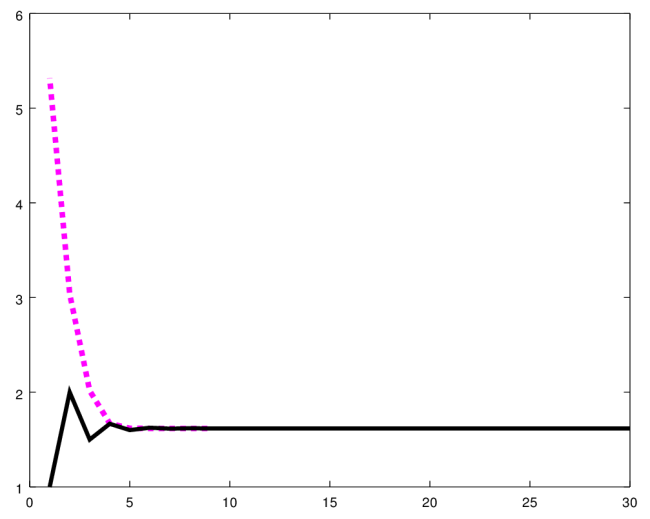
\includegraphics[scale=0.5]{phi2.png}
				\caption{Comparativo da convergência entre método de newton(pontilhado) com frações continuadas(continuo)}
				\label{fig:phi-graphic}
			\end{figure}

			Para gerarmos a tabela de resultados e o gráfico, foi usado o número
			\emph{6} como aproximação inicial no método de newton. No método de
			frações continuadas foi dado um limite de iterações de \emph{30} e
			em ambos os métodos o erro toleravel é de $10^{-12}$.

	\subsection{Pi($\pi$)}

		\subsubsection{Método Utilizando Funções Trigonométricas}

			Encontramos em um forum de matemática~\cite{mathForum} um método
			iterativo que calcula $\pi$ de uma forma aparentemente mais simples,
			apesar de sua complexidade estar escondida na função \emph{sin}. O
			método está descrito a seguir:

			\begin{equation}
			\label{magic_equation}
				P(n) =
				\begin{cases}
					3 + sin (3) & \quad \text{se } n \text{\ for } 1\\
					P(n-1) + sin(P(n-1)) & \quad \text{se } n > 1\\
				\end{cases}
			\end{equation}

			$P(n)$ seria a aproximação de $\pi$ na iteração $n$. Na primeira
			iteração, precisamos oferecer uma aproximação inicial. No nosso caso
			utilizamos \emph{3}, como podemos ver na
			equação~\ref{magic_equation}.

			Esse método consegue convergir para $\pi$ com um número muito baixo
			de iterações.

			\begin{table}[H]
\centering 
\begin{tabular}{|c|c|c|c|}
\hline 
Iteração & Aproximação & pi & Erro \\ 
\hline 
1 & 3.14112000805987e+00 &  3.14159265358979e+00 & 4.72645529925764e-04 \\ 
\hline
2 & 1.84147098480790e+00 &  3.14159265358979e+00 & 2.14159265358979e+00 \\ 
\hline
3 & 3.14159265357220e+00 &  3.14159265358979e+00 & 4.72645529925764e-04 \\ 
\hline
4 & 3.14159265358979e+00 &  3.14159265358979e+00 & 0.00000000000000e+00 \\ 
\hline
\end{tabular}
\label{table:pi-sin}
\caption{Convergência de pi utilizando funções trigonométricas}
\end{table}

			Os valores foram obtidos a partir do algoritmo abaixo:

			\begin{lstlisting}

				function pi_sin(iteration=1, err=1*10^-1)

					x(1,1) = 1
					x(2,1) = 3 + sin(3)
					x(3,1) = pi
					x(4,1) = abs(pi - x(2,1))
					i = 2
					while xor(i <= iteration,  err > x(4, i-1))
						x(1,i) = i
						x(2,i) = x(i-1) + sin(x(i-1))
						x(3,i) = pi
						x(4,i) = abs(pi - x(i-1))
						i++
					end

				end

			\end{lstlisting}

	\subsection{$e^x$}

		A função $e^x$ é um função exponencial cuja base é o número de Euler,
		também conhecida como função exponencial natural.

		Para o cálculo da da função utilizamos a seguinte série de Taylor

		\begin{equation}
			\sum_{n=1}^{n} = \frac{x^n}{n!}
		\end{equation}

		Para gerarmos os resultados da Tabela~\ref{table:exponential},
		utilizamos \emph{40} como limite máximo de iterações e $10^{-15}$ como erro
		tolerável.

		\begin{table}[H]
\centering 
\begin{tabular}{|c|c|c|c|}
\hline 
Iteração & Aproximação & $e^x$ & Erro \\ 
\hline 
1 & 1.00000000000000e+00 &  1.48413159102577e+02 & 1.47413159102577e+02 \\ 
\hline
2 & 6.00000000000000e+00 &  1.48413159102577e+02 & 1.47413159102577e+02 \\ 
\hline
3 & 1.85000000000000e+01 &  1.48413159102577e+02 & 1.42413159102577e+02 \\ 
\hline
4 & 3.93333333333333e+01 &  1.48413159102577e+02 & 1.29913159102577e+02 \\ 
\hline
5 & 6.53750000000000e+01 &  1.48413159102577e+02 & 1.09079825769243e+02 \\ 
\hline
6 & 9.14166666666667e+01 &  1.48413159102577e+02 & 8.30381591025766e+01 \\ 
\hline
7 & 1.13118055555556e+02 &  1.48413159102577e+02 & 5.69964924359099e+01 \\ 
\hline
8 & 1.28619047619048e+02 &  1.48413159102577e+02 & 3.52951035470210e+01 \\ 
\hline
9 & 1.38307167658730e+02 &  1.48413159102577e+02 & 1.97941114835290e+01 \\ 
\hline
10 & 1.43689456569665e+02 &  1.48413159102577e+02 & 1.01059914438464e+01 \\ 
\hline
11 & 1.46380601025132e+02 &  1.48413159102577e+02 & 4.72370253291169e+00 \\ 
\hline
12 & 1.47603848504890e+02 &  1.48413159102577e+02 & 2.03255807744432e+00 \\ 
\hline
13 & 1.48113534954789e+02 &  1.48413159102577e+02 & 8.09310597686419e-01 \\ 
\hline
14 & 1.48309568204750e+02 &  1.48413159102577e+02 & 2.99624147787284e-01 \\ 
\hline
15 & 1.48379580079737e+02 &  1.48413159102577e+02 & 1.03590897826081e-01 \\ 
\hline
16 & 1.48402917371399e+02 &  1.48413159102577e+02 & 3.35790228399446e-02 \\ 
\hline
17 & 1.48410210275043e+02 &  1.48413159102577e+02 & 1.02417311778993e-02 \\ 
\hline
18 & 1.48412355246703e+02 &  1.48413159102577e+02 & 2.94882753351544e-03 \\ 
\hline
19 & 1.48412951072164e+02 &  1.48413159102577e+02 & 8.03855873414250e-04 \\ 
\hline
20 & 1.48413107868338e+02 &  1.48413159102577e+02 & 2.08030412267135e-04 \\ 
\hline
21 & 1.48413147067382e+02 &  1.48413159102577e+02 & 5.12342382705810e-05 \\ 
\hline
22 & 1.48413156400487e+02 &  1.48413159102577e+02 & 1.20351947714425e-05 \\ 
\hline
23 & 1.48413158521648e+02 &  1.48413159102577e+02 & 2.70208917640957e-06 \\ 
\hline
24 & 1.48413158982770e+02 &  1.48413159102577e+02 & 5.80928826821037e-07 \\ 
\hline
25 & 1.48413159078837e+02 &  1.48413159102577e+02 & 1.19806998100103e-07 \\ 
\hline
26 & 1.48413159098050e+02 &  1.48413159102577e+02 & 2.37399433444807e-08 \\ 
\hline
27 & 1.48413159101745e+02 &  1.48413159102577e+02 & 4.52652670901443e-09 \\ 
\hline
28 & 1.48413159102429e+02 &  1.48413159102577e+02 & 8.31647639643052e-10 \\ 
\hline
29 & 1.48413159102551e+02 &  1.48413159102577e+02 & 1.47423406815506e-10 \\ 
\hline
30 & 1.48413159102572e+02 &  1.48413159102577e+02 & 2.52384779741988e-11 \\ 
\hline
31 & 1.48413159102576e+02 &  1.48413159102577e+02 & 4.17799128626939e-12 \\ 
\hline
32 & 1.48413159102576e+02 &  1.48413159102577e+02 & 6.53699316899292e-13 \\ 
\hline
33 & 1.48413159102577e+02 &  1.48413159102577e+02 & 8.52651282912120e-14 \\ 
\hline
34 & 1.48413159102577e+02 &  1.48413159102577e+02 & 0.00000000000000e+00 \\ 
\hline
\end{tabular}
\caption{Convergência de $e^x$ utilizando série de Taylor}
\label{table:erdos}
\end{table}

		Utilizando a série de Taylor foi percebido que o método converge após 24
		iterações.A complexidade desse método encontra-se no cáculo de
		\emph{n!}.

		Utilizamos o Algoritmo exponential implementado como mostrado a seguir,
		que retorna uma matriz de forma que cada coluna representa uma iteração
		e a primeira linha o valor calculado, a segunda o valor de $e^5$ e a
		tereceira linha é utilizada para guardar a diferença entre $e^5$ o valor
		calculado na iteração.

		\newpage

		\begin{lstlisting}
		function exponential(p, iteration, err)
			x(1,1) = 1
			x(2,1) = 1
			x(3,1) = e^p
			x(4,1) = abs(e^p - x(2,1))

			i=2
			while xor(i <= iteration,  err > x(4, i-1))
				x(1,i) = i
				x(2,i) = x(2,i-1) + (power(p,i-1)) / (factorial(i-1))
				x(3,i) = e^p
				x(4,i) = abs(x(3,i) - x(2,i-1))
				i++
			end
		end
		\end{lstlisting}

	\subsection{Erdős-Borwein}

		A constante de Erdős-Borwein é a soma dos inversos multiplicativos dos
		números de Mersenne, e por definição é:

		\begin{equation}
			E = \displaystyle\sum_{n=1}^{\infty} \frac{1}{2^n-1} \approx 1.606695152415291763\dots
		\end{equation}

		Executando no ambiente matemático \emph{octave}, obtemos os seguintes
		resultados:

		\begin{table}[H]
\centering 
\begin{tabular}{|c|c|c|c|}
\hline 
Iteração & Aproximação & Erro \\ 
\hline 
1 & 1.00000000000000e+00 &  6.06695152415292e-01 \\ 
\hline
2 & 1.33333333333333e+00 &  6.06695152415292e-01 \\ 
\hline
3 & 1.47619047619048e+00 &  2.73361819081958e-01 \\ 
\hline
4 & 1.54285714285714e+00 &  1.30504676224816e-01 \\ 
\hline
5 & 1.57511520737327e+00 &  6.38380095581490e-02 \\ 
\hline
6 & 1.59098822324629e+00 &  3.15799450420200e-02 \\ 
\hline
7 & 1.59886223899432e+00 &  1.57069291690042e-02 \\ 
\hline
8 & 1.60278380762177e+00 &  7.83291342097270e-03 \\ 
\hline
9 & 1.60474075478420e+00 &  3.91134479352173e-03 \\ 
\hline
10 & 1.60571827189075e+00 &  1.95439763109517e-03 \\ 
\hline
11 & 1.60620679167580e+00 &  9.76880524545809e-04 \\ 
\hline
12 & 1.60645099192000e+00 &  4.88360739494542e-04 \\ 
\hline
13 & 1.60657307713548e+00 &  2.44160495294299e-04 \\ 
\hline
14 & 1.60663411601725e+00 &  1.22075279813894e-04 \\ 
\hline
15 & 1.60666463452672e+00 &  6.10363980462214e-05 \\ 
\hline
16 & 1.60667989354862e+00 &  3.05178885702251e-05 \\ 
\hline
17 & 1.60668752300136e+00 &  1.52588666735287e-05 \\ 
\hline
18 & 1.60669133771318e+00 &  7.62941393417371e-06 \\ 
\hline
19 & 1.60669324506545e+00 &  3.81470211663348e-06 \\ 
\hline
20 & 1.60669419874067e+00 &  1.90734984584218e-06 \\ 
\hline
21 & 1.60669467557806e+00 &  9.53674619941225e-07 \\ 
\hline
22 & 1.60669491399669e+00 &  4.76837234364424e-07 \\ 
\hline
23 & 1.60669503320600e+00 &  2.38418598419443e-07 \\ 
\hline
24 & 1.60669509281065e+00 &  1.19209294657807e-07 \\ 
\hline
25 & 1.60669512261297e+00 &  5.96046463297029e-08 \\ 
\hline
26 & 1.60669513751413e+00 &  2.98023230538291e-08 \\ 
\hline
27 & 1.60669514496471e+00 &  1.49011616379369e-08 \\ 
\hline
28 & 1.60669514869000e+00 &  7.45058104101304e-09 \\ 
\hline
29 & 1.60669515055265e+00 &  3.72529074255112e-09 \\ 
\hline
30 & 1.60669515148397e+00 &  1.86264559332017e-09 \\ 
\hline
31 & 1.60669515194963e+00 &  9.31323018704688e-10 \\ 
\hline
32 & 1.60669515218246e+00 &  4.65661731396949e-10 \\ 
\hline
33 & 1.60669515229888e+00 &  2.32831087743079e-10 \\ 
\hline
34 & 1.60669515235708e+00 &  1.16415765916145e-10 \\ 
\hline
35 & 1.60669515238619e+00 &  5.82081050026773e-11 \\ 
\hline
36 & 1.60669515240074e+00 &  2.91042745459436e-11 \\ 
\hline
37 & 1.60669515240802e+00 &  1.45523593175767e-11 \\ 
\hline
38 & 1.60669515241165e+00 &  7.27640170339328e-12 \\ 
\hline
39 & 1.60669515241347e+00 &  3.63842289630156e-12 \\ 
\hline
40 & 1.60669515241438e+00 &  1.81943349275571e-12 \\ 
\hline
41 & 1.60669515241484e+00 &  9.09938790982778e-13 \\ 
\hline
42 & 1.60669515241506e+00 &  4.55191440096314e-13 \\ 
\hline
43 & 1.60669515241518e+00 &  2.27817764653082e-13 \\ 
\hline
44 & 1.60669515241523e+00 &  1.14130926931466e-13 \\ 
\hline
45 & 1.60669515241526e+00 &  5.72875080706581e-14 \\ 
\hline
\end{tabular}
\caption{Convergência de Erdős-Borwein}
\label{table:erdos}
\end{table}

		A definição de $E$ foi codificada da seguinte maneira:

		\begin{lstlisting}

			function erdos(iteration, err)
				erds   = 1.6066951524152917
				x(1,1) = 1
				x(2,1) = 1
				x(3,1) = abs(erds - x(2,1))

				i=2
				while xor(i <= iteration,  err > x(3, i-1))
					x(1,i) = i
					x(2,i) = x(2,i-1) + (1 / ((2^i)-1))
					x(3,i) = abs(erds - x(2,i-1))
					i++
				end
			end

		\end{lstlisting}

\section{Conclusão}
\label{sec:conclusao}

	Métodos iterativos são extremamente importantes dentro da computação, pois eles
	nos permitem aproximar números irracionais, com precisão aceitável a ser usada
	no sistema de ponto flutuante dentro dos computadores. Observamos que diferentes
	métodos possuem diferentes características que podem complicar ou simplificar em
	alguns aspectos. Como na equação~\ref{magic_equation}, onde aparenta ser
	simples, mas a complexidade está escondida dentro da função \emph{sin}, que por
	sua vez, é implementada utilizando série de taylor por trás.


\bibliographystyle{sbc}
\bibliography{bibliografia}

\end{document}
